\documentclass[working, oneside]{../../../Preambles/tuftebook}
% Import xcolor and define some colors
\usepackage{{xcolor}}
\definecolor{{background}}{{HTML}}{{{background}}}
\definecolor{{foreground}}{{HTML}}{{{foreground}}}
\definecolor{{math}}{{HTML}}{{{color6}}}

%%%%%%%%%%%%%%%%%%%%%%%%%%%%%%%%%%%%%%%% IMPORTS %%%%%%%%%%%%%%%%%%%%%%%%%%%%%%%%%%%%%%%%
\documentclass[11pt,onesize,a4paper,titlepage]{article}

%%%%%%%%%%%%%%% Formatting %%%%%%%%%%%%%%% 
\usepackage[english]{babel}
\usepackage[utf8]{inputenc}
\usepackage{adjustbox}
\usepackage{geometry} % Margins
\usepackage{sectsty} % Custom Sections

%%%%%%%%%%%%%%% Font %%%%%%%%%%%%%%% 
\usepackage{Archivo}
\usepackage[T1]{fontenc}
\sffamily

%%%%%%%%%%%%%%% Graphics %%%%%%%%%%%%%%% 
\usepackage{fontawesome5} % Icons
\usepackage{graphicx} % Images
\usepackage[most]{tcolorbox} % Color Box
\usepackage{xcolor} % Colors
\usepackage{tikz} % For Drawing Shapes
%%%\usepackage{emoji} % For flags
\tcbuselibrary{breakable}
%%%\usepackage{academicons}

%%%%%%%%%%%%%%% Miscelanous %%%%%%%%%%%%%%% 
\usepackage{lipsum} % Lorem Ipsum
\usepackage{hyperref} % For Hyperlinks

%%%%%%%%%%%%%%% Colors %%%%%%%%%%%%%%% 
\definecolor{title}{HTML}{b5bff5} % Color of the title
\definecolor{bars}{HTML}{889af0} % Color of the title
\definecolor{backdrop}{HTML}{f2f2f2} % Color of the side column
\definecolor{lightgray}{HTML}{dfdfdf} % Color for the skill bars

%%% TU green: #639a00
%%% TU gray: #e6e6e6
%\definecolor{title}{HTML}{639a00} % Color of the title TU
%\definecolor{bars}{HTML}{889af0} % Color of the title TU

% \definecolor{backdrop}{HTML}{f2f2f2} % Color of the side column
\definecolor{backdrop}{HTML}{e6e6e6} % Color of the side column

\definecolor{subtitle}{HTML}{606060} % 


%%%%%%%%%%%%%%% Section Format %%%%%%%%%%%%%%% 
\sectionfont{                     
    \LARGE % Font size
    \sectionrule{0pt}{0pt}{-8pt}{1pt} % Rule under Section name
}

\subsectionfont{
    \Large % Font size
    \fontfamily{phv}\selectfont % Font family
    %\sectionrule{0pt}{0pt}{-8pt}{1pt} % Rule under Subsection name
    \sectionrule{5pt}{0pt}{0pt}{0pt} % Rule under Subsection name
}

%%%%%%%%%%%%%%% Margins and Headers %%%%%%%%%%%%%%%
\geometry{
  a4paper,
  left=7mm,
  right=7mm,
  bottom=10mm,
  top=10mm
}

\pagestyle{empty} % Empty Headers

\usepackage{marvosym}

% \renewcommand\qedsymbol{\CoffeeCup}

\usepackage{changepage}

\newenvironment{subexercise}[1]{%
    \begin{mdframed}[linewidth=0.5pt, linecolor=foreground, backgroundcolor=background, leftmargin=0cm, innerleftmargin=1em, innertopmargin=0pt, innerbottommargin=0pt, innerrightmargin=0pt, topline=false, rightline=false, bottomline=false]
    \par\noindent\textcolor{foreground}{\textbf{#1.}}\hspace{1em}\ignorespaces
}{%
    \par\addvspace{\baselineskip}\end{mdframed}\ignorespacesafterend
}
\newenvironment{solution}{%
    % \par\addvspace{\baselineskip}\noindent\makebox[\textwidth]{\textcolor{foreground}{\textbullet\hspace{1em}\textbullet\hspace{1em}\textbullet}}\par\addvspace{\baselineskip}
    \begin{mdframed}[linewidth=0.5pt, linecolor=foreground, backgroundcolor=background, rightmargin=0cm, innerleftmargin=0cm, innertopmargin=0pt, innerbottommargin=0pt, innerrightmargin=1em, topline=false, leftline=false, bottomline=false]
    \par\noindent\textcolor{foreground}{\textit{Solution.}}\hspace{1em}\ignorespaces
}{%
    \par\addvspace{\baselineskip}\noindent\hfill\textcolor{foreground}{\Coffeecup}\par\addvspace{\baselineskip}\end{mdframed}\ignorespacesafterend
}
% Exercise environment

\declaretheoremstyle[
    name= \textcolor{foreground}{Exercise},
    postheadspace = \newline,
    bodyfont = \normalfont\color{foreground},
    postheadhook={\textcolor{math}{\rule[.4ex]{\linewidth}{0.5pt}}\\},
    % numberwithin=chapter,
    mdframed={
        backgroundcolor = background,
        linecolor = foreground,
        linewidth = 0.5pt,
        rightline =  true,
        topline = true,
        bottomline = true,
        skipabove=20pt,
        skipbelow=20pt,
        innerleftmargin=15pt,
        innertopmargin=10pt,
        innerrightmargin=15pt,
        innerbottommargin=10pt}
    ]{exercise}
\declaretheorem[style=exercise,numbered=no]{exercise}

% \etocsetlevel{exercise}{2}

% \AtEndEnvironment{exercise}{%
%   \etoctoccontentsline{exercise}{\protect\numberline{\theexercise}}%
% }%
% \etocsetstyle{exercise}
% {}
% {}
% % this will be rendered like a non-numbered section, but we could have used
% % \numberline here also
% {\etocsavedsectiontocline{Exercise \etocnumber}{\etocpage}}
%     {}

% theorem environment

\declaretheoremstyle[
    name= \textcolor{foreground}{Theorem},
    postheadspace = \newline,
    bodyfont = \normalfont\color{foreground},
    postheadhook={\textcolor{math}{\rule[.4ex]{\linewidth}{1pt}}\\},
    mdframed={
        backgroundcolor = background,
        linecolor = foreground,
        linewidth = 1pt,
        rightline =  true,
        topline = true,
        bottomline = true,
        skipabove=20pt,
        skipbelow=20pt,
        innerleftmargin=15pt,
        innertopmargin=10pt,
        innerrightmargin=15pt,
        innerbottommargin=10pt}
    ]{theorem}
\declaretheorem[style=theorem,numbered=yes]{theorem}

\declaretheoremstyle[
    name= \textcolor{foreground}{Definition},
    postheadspace = \newline,
    bodyfont = \normalfont\color{foreground},
    postheadhook={\textcolor{math}{\rule[.4ex]{\linewidth}{1pt}}\\},
    mdframed={
        backgroundcolor = background,
        linecolor = foreground,
        linewidth = 1pt,
        rightline =  true,
        topline = true,
        bottomline = true,
        skipabove=20pt,
        skipbelow=20pt,
        innerleftmargin=15pt,
        innertopmargin=10pt,
        innerrightmargin=15pt,
        innerbottommargin=10pt}
    ]{definition}
\declaretheorem[style=definition,numbered=yes]{definition}
% Example environment

\declaretheoremstyle[
name= \quad \underline{Proof:},
     headfont = \bfseries\sffamily,
     postheadspace = \newline,
     % notebraces = \bfseries{(}{)a},
     headpunct = {},
     bodyfont = ,
     postheadhook={\textcolor{foreground}{\rule[0.4ex]{\linewidth}{0pt}}\\},
     qed=\qedsymbol,
    % spacebelow = 10pt,
    mdframed={
  backgroundcolor = background,
  linecolor = foreground,
  linewidth = 1pt,
  skipabove=10pt,
  skipbelow=10pt,
  rightline = false,
  topline = false,
  leftline = false,
  bottomline = false,
  innerleftmargin=15pt,
  innertopmargin=15pt,
  innerrightmargin=15pt,
  innerbottommargin=15pt}
]{pro}
    % \declaretheorem[style=pro,numbered=no]{Proof}

\declaretheoremstyle[
name= \quad \underline{\textcolor{foreground}{Example}},
     headfont = \bfseries\sffamily,
     postheadspace = \newline,
     % notebraces = \bfseries{(}{)a},
     headpunct = {},
     bodyfont = \normalfont\color{foreground},
     postheadhook={\textcolor{foreground}{\rule[0.4ex]{\linewidth}{0pt}}\\},
     % spacebelow = 10pt,
    mdframed={
  backgroundcolor = background,
  linecolor = foreground,
  linewidth = 1pt,
  skipabove=10pt,
  skipbelow=10pt,
  rightline = false,
  topline = false,
  leftline = false,
  bottomline = false,
  innerleftmargin=15pt,
  innertopmargin=15pt,
  innerrightmargin=15pt,
  innerbottommargin=15pt}
]{ex}
\declaretheorem[style=ex,numbered=no]{example}

\declaretheoremstyle[
     name=,
     headfont = \bfseries\sffamily,
     notebraces = \bfseries{},
     headpunct = { -},
     bodyfont = \color{foreground}\normalfont,
     % postheadhook={\textcolor{black}{\rule[.4ex]{\linewidth}{0.2pt}}\\},
    % spacebelow = 10pt,
    mdframed={
  backgroundcolor = background,
  linecolor = foreground,
  linewidth = 1pt,
  skipabove=0pt,
  skipbelow=0pt,
  innerleftmargin=10pt,
  innertopmargin=10pt,
  innerrightmargin=10pt,
  innerbottommargin=10pt,
  rightline = false,
  topline = false,
  leftline = false,
  bottomline = true}
]{subexercise}
% \declaretheorem[style=subexercise,numbered=no]{subexercise}

\declaretheoremstyle[
     name= \color{losning}Løsning,
     headfont = \bfseries\sffamily,
     notebraces = \bfseries{},
     postheadspace = \newline,
     headpunct = {:},
     bodyfont = \normalfont,
     % qed = ,
     % postheadhook={\textcolor{black}{\rule[.4ex]{\linewidth}{0.2pt}}\\},
    % spacebelow = 10pt,
    mdframed={
  backgroundcolor = background,
  linecolor = losning!75,
  linewidth = 1pt,
  skipabove=0pt,
  skipbelow=10pt,
  innerleftmargin=10pt,
  innertopmargin=10pt,
  innerrightmargin=10pt,
  innerbottommargin=10pt,
  leftline = false,
  rightline = true,
  topline = false,
  bottomline = true}
]{solution}

\newenvironment{SimpleBox}[1]{%
  \begin{mdframed}%
    \noindent\textbf{#1}\\[1ex]
}{%
  \end{mdframed}%
}


\begin{document}
\let\cleardoublepage\clearpage
\thispagestyle{fancy}
\chapter{Aflevering 1 - Databaser}
\begin{exercise}[1]
Create and provide short explanations for an E/R diagram that
\begin{itemize}
    \item[i.] has at least four entity sets, and at most 8 relevant attributes. You should also have
relationship sets between appropriate entity sets. 
\item[ii.] provide primary keys (making use of existing attributes in the diagram, so not via artificial
identifiers like “ID”).
\item[iii.] contains a weak entity set - why is it weak?
\item[iv.] note cardinality ratios use any syntax – Explain the chosen cardinality ratio for at least one relationship set.
\end{itemize}
\end{exercise}
I have created the following ER-diagram for the NGO.
\begin{figure}[htpb]
    \centering
    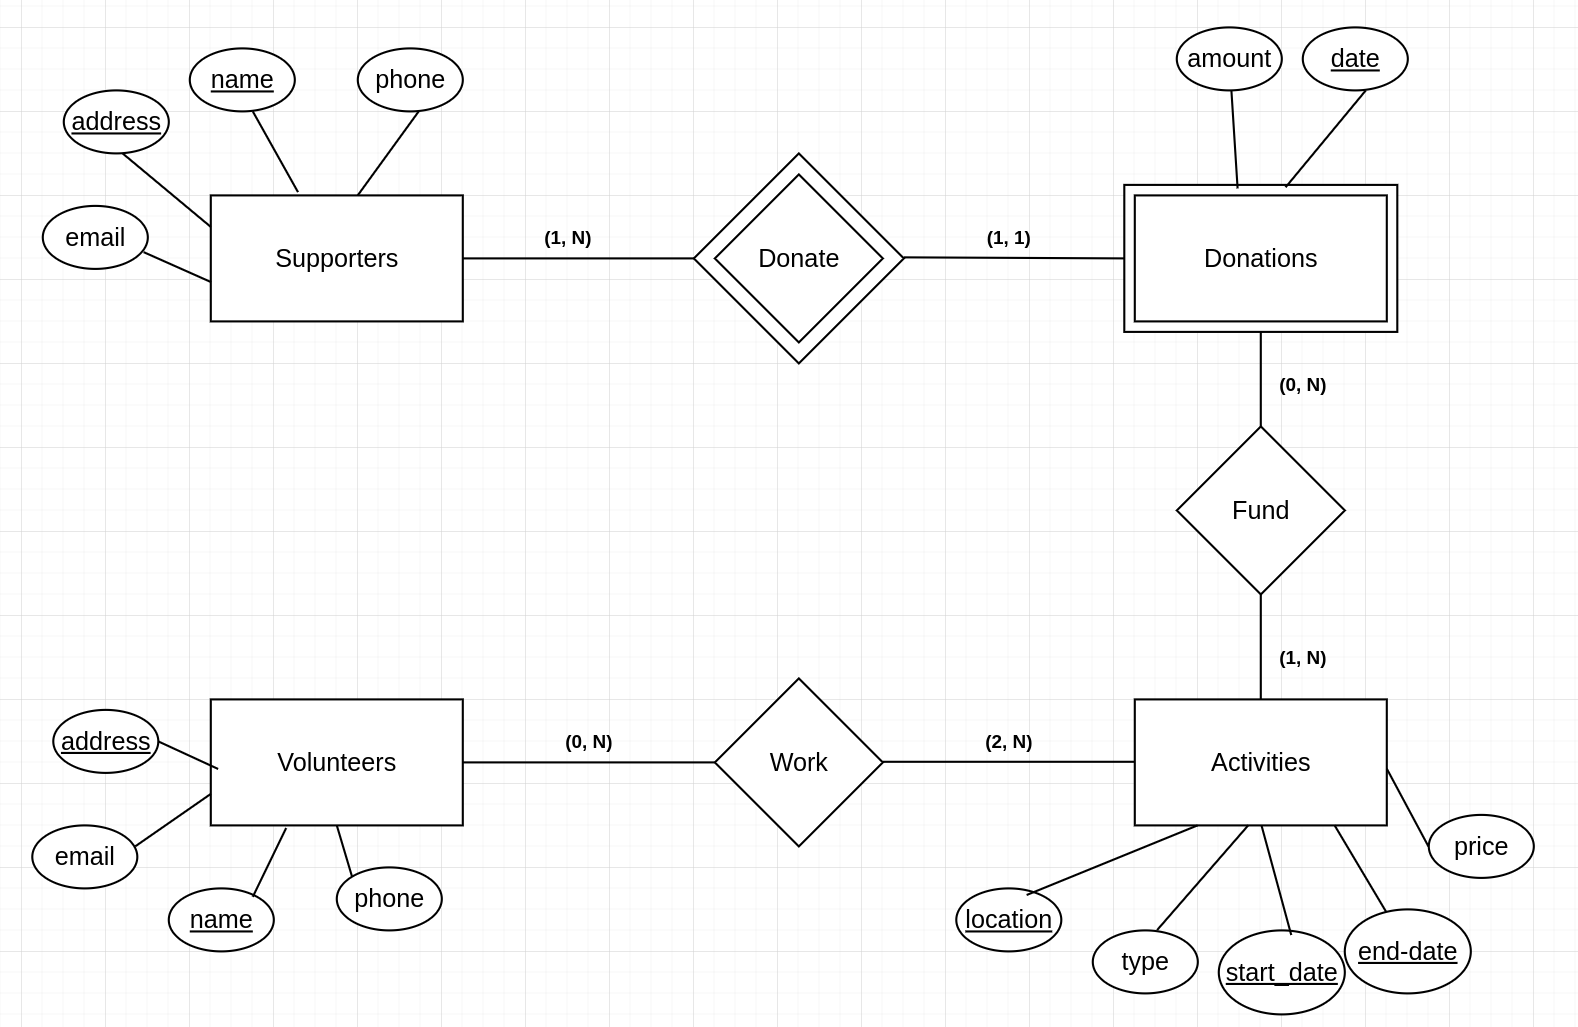
\includegraphics[width=0.8\textwidth]{../afl_1/Screenshot from 2025-02-13 11-54-44.png}
\end{figure}
It has the following four entity sets: Supporters, Donations, Activities and Volunteers. The relationship sets: Work, Fund and Donate, describe the relationships between the entity sets. My idea of an NGO is that it receives donations from supporters and uses said donations to fund a variety of different charitable activities. For the supporters i have stored their contact information as attributes. The primary key is (name, address), I think it is reasonable to assume that we wont have two supporters with the same name who live on the same address. Donations is a weak entity which is supported by Supporters. It has as its primary key the date of the donation and amount combined with the primary key of Supporters as a foreign key. I have here assumed that a supporter wont make more than one donation of the same amount per day. I think this is reasonable aswell.
\\
The cardinality ratio between Supporters and Donations are (1, N) and (1, 1) respectively. In other words, a supporter has to make at least one donation to be included in the donation, but can make as many as they want. On the other hand a donation, stems from a single supporter and every donation should have a supporter listed. This makes sense intuitively, but is also required as Donations is a weak entity set.
\\
The cardinality ratio between Volunteers and Activities is (0, N) and (2, N). A volunteer can sign up for the NGO, without commiting to an activity, while an activity should have at least 2 volunteers assigned to it. In the same way, donations arent assigned to activities immediately, but activities should have funding secured.
\begin{exercise}[2]
 Create a database schema from this E/R diagram. Explain how you did this for
 \begin{itemize}
\item[i.] at least one entity set
\item[ii.] at least one relationship set
\item[iii.] at least one attribute
\item[iv.] discuss for at least one example of how you used the cardinality ratios to determine the schema
 \end{itemize}
\end{exercise}
In converting the ER-diagram to a schema, I made use of the rules given in the lectures. Entities are converted to tables, with attributes as elements. Relationships are also converted to tables, but have keys from their related entities as elements. Weak entities borrow the keys from their supporting sets. I then get the following schema.
\begin{align*}
    Supporters :& (\underline{name}, \underline{address}, phone, email) \\
    Donations :& (\underline{amount}, \underline{date}, \#name, \#name) \\
    Activities :& (\underline{location}, \underline{start\_ date},\underline{end\_ date}, price, type) \\
    Volunteers :& (\underline{name}, \underline{address}, phone, email) \\
    Work :& (\underline{name}, \underline{address},\underline{location}, \underline{start\_ date},\underline{end\_ date}) \\
Fund :& (\underline{location}, \underline{start\_date}, \underline{end\_date}, \underline{date}, \underline{name}, \underline{address})
.\end{align*}
For the entity sets, the tables are straightforward. Their primary key is underlined, and all attributes are included as elements. The Fund table is a relationship between Activity and the weak entity Donations, so it has to include the primary key of Donations' supporting entity. Due to the cardinality ratio (1, 1) between Donations and Supporters, i can merge Donate into Donations, as the Donate would table would have been a proper subset of Donations.
\begin{exercise}[3]

\end{exercise}
\end{document}
